% Figure 1: Biome data pipeline schematic
\begin{figure}[htbp]
\centering

\includegraphics[width=0.95\textwidth]{figures/fig_workflow.pdf}
\caption{Biome data pipeline. Users upload photographs with EXIF metadata; a convolutional species-identification model refined by geospatial priors produces a candidate list, which can be confirmed directly or submitted for community identification via the ``Ask Biomers'' feature. Automatic filtering (non-wild labels, private records, cultural-centre locations, certified-user gating: $<$15\% misidentification rate, $<$0.5\% inappropriate records, $>$20 public records) retained 2{,}373{,}303 of 5{,}275{,}457 records (45.0\%) for downstream species distribution modelling.}
\label{fig:workflow}
\end{figure}

% Figure 2: Taxonomic composition of Biome records
\begin{figure}[htbp]
\centering
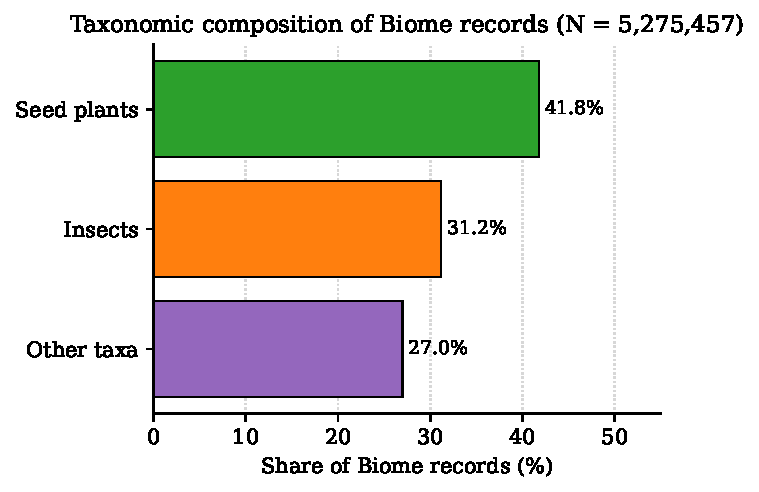
\includegraphics[width=0.75\textwidth]{figures/fig_taxa_composition.pdf}
\caption{Taxonomic composition of the 5{,}275{,}457 records submitted to Biome by 7 July 2023. Seed plants (41.8\%) and insects (31.2\%) dominate the submissions, reflecting their accessibility to smartphone photography. The remaining 27.0\% aggregates all other taxa (birds, mammals, reptiles, amphibians, fishes, molluscs, arthropods, non-seed plants, and other invertebrates).}
\label{fig:taxa}
\end{figure}

% Figure 3: Training records required to reach BI > 0.9
\begin{figure}[htbp]
\centering
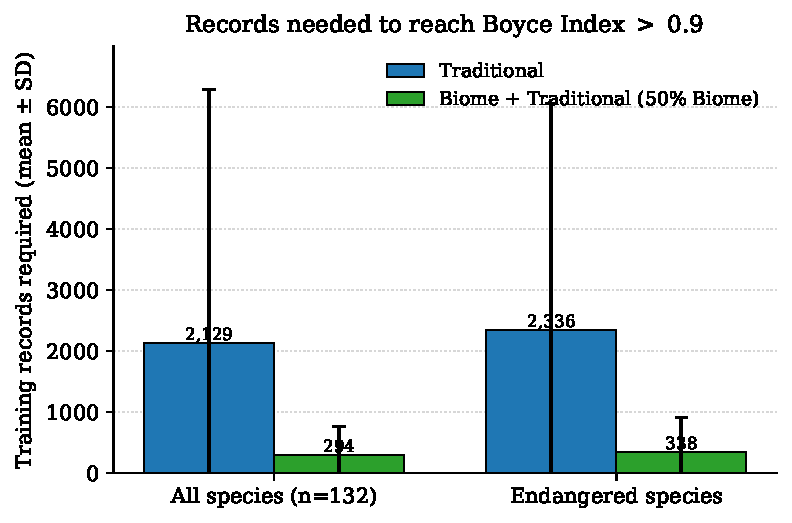
\includegraphics[width=0.8\textwidth]{figures/fig_records_to_bi09.pdf}
\caption{Training records required for species distribution models to exceed a Boyce Index of 0.9. For all 132 modelled species, Traditional survey data require 2{,}129 $\pm$ 4{,}157 records (mean $\pm$ SD) to reach the threshold, whereas Biome+Traditional data (50\% Biome) require only 294 $\pm$ 471 records. For endangered species listed on Japan's national or prefectural red lists, the corresponding requirements are 2{,}336 $\pm$ 3{,}718 and 338 $\pm$ 571 records.}
\label{fig:records}
\end{figure}

% Figure 4: Best per-species Boyce Index
\begin{figure}[htbp]
\centering
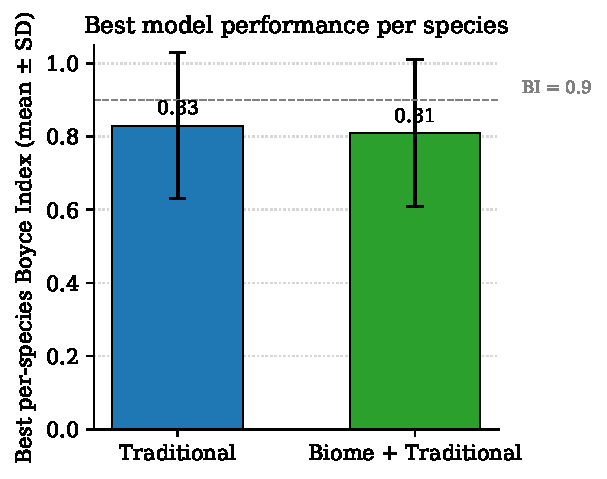
\includegraphics[width=0.6\textwidth]{figures/fig_best_bi.pdf}
\caption{Best Boyce Index attained per species under each training regime. When each dataset is allowed its full data budget, the best per-species accuracy is statistically indistinguishable (Traditional: $0.83 \pm 0.20$; Biome+Traditional: $0.81 \pm 0.20$; mean $\pm$ SD across 132 species). The advantage of Biome blending therefore lies in the amount of data required to reach a given accuracy rather than in the ceiling performance.}
\label{fig:bestbi}
\end{figure}
